\documentclass[docmute]{article}

\usepackage[margin=1in]{geometry}


% AMS packages for enhanced math typesetting and symbols:
\usepackage{amsmath}  % Provides enhanced math features like align, gather, etc.
\usepackage{amssymb}  % Provides additional math symbols
\usepackage{amsthm}   % Enables theorem-like environments

\usepackage{graphicx} % Provides commands for including and managing external graphics (e.g., figures, images)

% Package for customizing list environments:
\usepackage{enumitem} % Allows control over layout of lists (itemize, enumerate, etc.)

% Full-page layout package:
\usepackage{fullpage} % Uses more of the page area by reducing margins

% TikZ package for drawing graphics:
\usepackage{tikz}     % Used for creating high-quality diagrams and figures

% Microtype package for typographical enhancements:
\usepackage{microtype} % Improves justification, kerning, and overall appearance

% Package for typesetting polynomials:
\usepackage{polynom}  % Provides commands for polynomial long division and related tasks

% Package for controlling figure placement:
\usepackage{placeins} % Provides the \FloatBarrier command to control floating environments

% Forest package for drawing trees:
\usepackage{forest}   % Simplifies the creation of tree diagrams

% Package to allow one LaTeX file to input another:
\usepackage{docmute}  % Allows this file to be included in another document without reloading the preamble

% Load additional TikZ libraries:
\usetikzlibrary{trees} % Provides additional tree-specific commands for TikZ

% Define theorem-like environments using amsthm:
\newtheorem{corollary}{Corollary} % Defines a new "corollary" environment
\newtheorem{lemma}{Lemma}         % Defines a new "lemma" environment

\input{watermark/watermark.tex}

\title{Introduction to Coding Theory}
\author{Tomasz Brengos \\  
Committers : Aliaksei Kudzelka, Mykhailo Moroz}
\date{}

\begin{document}
\maketitle


\section{Encoding and Decoding Functions}

Let $p$ be a prime number. We work over the finite field $\mathbb{Z}_p$ (the integers mod $p$). For any positive integer $n$, the set $\mathbb{Z}_p^n$ denotes the set of all $n$-tuples of elements from $\mathbb{Z}_p$. Note that since $\mathbb{Z}_p$ is a field, the spaces $\mathbb{Z}_p^n$ and $\mathbb{Z}_p^k$ can be viewed as vector spaces (of dimension $n$ or $k$ respectively) over $\mathbb{Z}_p$.

\medskip

\noindent \textbf{Encoding function:} A map $\xi: \mathbb{Z}_p^k \to \mathbb{Z}_p^n$ is called an \emph{encoding function} (or \emph{coding function}) if it is one-to-one (distinct messages have distinct codewords). In other words, $\xi$ takes each possible message (an element of $\mathbb{Z}_p^k$) and encodes it as a longer string (an element of $\mathbb{Z}_p^n$). The image of $\xi$, denoted 
\[ \mathcal{C} = \xi(\mathbb{Z}_p^k) \subseteq \mathbb{Z}_p^n, \] 
is the set of all possible encoded messages and is called the \emph{code}. The elements of $\mathcal{C}$ are called \emph{codewords}. Working over the field $\mathbb{Z}_p$ is crucial here, because it ensures we can use the tools of linear algebra and arithmetic modulo $p$ when designing and analyzing codes.

\medskip

\noindent \textbf{Decoding function:} Given an encoding $\xi$, a map $\eta: \mathbb{Z}_p^n \to \mathbb{Z}_p^k$ is called a \emph{decoding function} for $\xi$ if $\eta(\xi(u)) = u$ for every $u \in \mathbb{Z}_p^k$. In other words, $\eta$ is a (left) inverse of $\xi$ on the set of codewords, so that decoding an encoded message returns the original message (assuming no errors in transmission).

\medskip

Once a message $u \in \mathbb{Z}_p^k$ is encoded as a codeword $c = \xi(u) \in \mathbb{Z}_p^n$, it is sent through a channel (transmission). During transmission, some components of $c$ might be altered due to noise or other errors.

\section{Error Vectors and Transmission Errors}

When a codeword is transmitted (over a noisy channel, or stored and later retrieved), some of its components may change due to errors. We can model the effect of errors by an \emph{error vector}. An \emph{error vector} \(\mathbf{e} \in \mathbb{Z}_p^n\) is a vector that, when added to the original codeword, yields the \emph{received word}. If \(\mathbf{c} \in \mathcal{C}\) is the sent codeword and \(\mathbf{e}\) is the error vector, then the received word is
\[
  \mathbf{r} = \mathbf{c} + \mathbf{e},
\]
where addition is component-wise in \(\mathbb{Z}_p\). (In the case \(p=2\), this addition is XOR of bits.) The nonzero entries of \(\mathbf{e}\) indicate positions where an error occurred (and the value indicates what was added at that position, e.g.\ a flip from 0 to 1 in binary is represented by adding 1 mod 2).

The number of errors that occur is the number of nonzero entries in \(\mathbf{e}\). This is called the \emph{weight} of \(\mathbf{e}\), often denoted \(w(\mathbf{e})\). If \(w(\mathbf{e}) = t\), we say \(t\) errors occurred. The coding and decoding process can be summarized as:
\[
  \mathbf{u} \xrightarrow{\xi} \mathbf{c}
            \xrightarrow{\text{error }\mathbf{e}}
            \mathbf{r} = \mathbf{c} + \mathbf{e}
            \xrightarrow{\eta} \hat{\mathbf{u}},
\]
where \(\hat{\mathbf{u}} = \eta(\mathbf{r})\) is the decoder’s estimate of the original message. We desire \(\hat{\mathbf{u}} = \mathbf{u}\) even if \(\mathbf{e}\) is nonzero (up to a certain weight). The design of \(\mathcal{C}\) and \(\eta\) determines how many errors can be reliably detected or corrected.


\section{Examples of Encoding Functions (Codes)}

We now present a few example encoding functions and their corresponding codes:

\subsection*{Example 1: Repetition Code}
One simple encoding is the \emph{repetition code}. Here the message space is $\mathbb{Z}_p$ (messages of length 1). The encoding function $\xi_1: \mathbb{Z}_p \to \mathbb{Z}_p^n$ for some chosen length $n$ is defined by 
\[ \xi_1(a) = (\underbrace{a, a, \ldots, a}_{n \text{ times}}), \] 
i.e. the single-symbol message $a$ is repeated $n$ times to form the codeword. The code $\mathcal{C}_1 = \{(a,a,\ldots,a) : a \in \mathbb{Z}_p\}$ consists of all $n$-tuples with identical entries. This encoding is one-to-one (different $a$ give different constant tuples).

\medskip

For example, over $\mathbb{Z}_2$ (the binary case), if $a=1$ and $n=5$, the codeword would be $(1,1,1,1,1)$. If a transmission error flips one of these bits (say we receive $(1,1,1,0,1)$), the decoder can notice that this is not a valid codeword in $\mathcal{C}_1$ (since not all bits are the same), hence an error is detected. In fact, the repetition code is able to detect up to $n-1$ errors (any change in at most $n-1$ positions will yield a tuple that is not constant and thus not in the code). This code even has error-correcting capability: intuitively, the decoder could guess that the majority value is the intended bit (for example, from $(1,1,1,0,1)$ a reasonable decoded value for $a$ would be 1, since most bits are 1). However, our focus here is on error detection criteria, which we formalize later.

\subsection*{Example 2: Parity Check Code}
Another useful encoding adds a \emph{parity check} to the message. For this example, let's work in $\mathbb{Z}_p$ (and especially consider $p=2$ for binary parity). Let the message space be $\mathbb{Z}_p^{\,k-1}$ (messages of length $k-1$). Define an encoding function $\xi_2: \mathbb{Z}_p^{\,k-1} \to \mathbb{Z}_p^k$ by 
\[ \xi_2(a_1, a_2, \ldots, a_{k-1}) = \big(a_1, a_2, \ldots, a_{k-1}, \; a_k\big), \] 
where the last component $a_k$ is chosen such that the total sum of the $k$ components is 0 in $\mathbb{Z}_p$. In other words,
\[ a_k \;=\; -\,(a_1 + a_2 + \cdots + a_{k-1}) \pmod{p}, \] 
which ensures $a_1 + a_2 + \cdots + a_{k-1} + a_k \equiv 0 \pmod{p}$. This extra symbol $a_k$ is a redundancy (the \emph{parity symbol}) chosen to enforce a constraint on every codeword.

The resulting code is 
\[ \mathcal{C}_2 = \{(a_1,\ldots,a_{k-1},a_k) \in \mathbb{Z}_p^k : a_1 + \cdots + a_{k-1} + a_k = 0\}. \] 
In the special case $p=2$ (binary), this encoding is the standard single-parity-bit code: the last bit $a_k$ is 0 or 1 chosen to make the total number of 1's in the codeword even. For example, if the message is $(1,0,1,1)$ in $\mathbb{Z}_2^4$ (so $k-1=4$), then the parity bit $a_5$ is chosen so that $1+0+1+1+a_5 \equiv 0 \pmod{2}$. Here $1+0+1+1 = 3 \equiv 1 \pmod{2}$, so we must take $a_5 = 1$ to make the sum even. The encoded 5-bit codeword is $(1,0,1,1,1)$, which has an even number of 1's (four 1's in this case).

This parity check code allows detection of any single-error in transmission: if one bit of a codeword is flipped, the parity (sum mod $p$) will no longer be zero, so the received word will violate the code constraint and thus be recognized as invalid. For instance, if $(1,0,1,1,1)$ is sent and one bit flips, the sum of bits will be odd, alerting us to the error. In fact, more generally, if an odd number of bits are in error, the parity check will detect it (sum becomes nonzero mod 2). However, if an even number of bits are corrupted in the binary case, the parity check could fail to detect it (since an even number of flips can restore the sum to even).

\subsection*{Example 3: \textsc{PESEL} Check Digit (revised)}
The Polish national identification number (\textsc{PESEL}) is an
11-digit string
\[
  YY\,MM\,DD\,PPPP\,K,
\]
where
\begin{itemize}
  \item $YYMMDD$ is the date of birth.  
  \item $PPPP$ is a serial number; its last digit is \emph{even} for
        females and \emph{odd} for males.
  \item $K$ is the check digit making
        \[
          \sum_{i=1}^{10} w_i\,p_i + K \equiv 0 \pmod{10},
          \quad
          (w_i)_{i=1}^{10}=1,3,7,9,1,3,7,9,1,3.
        \]
\end{itemize}

\paragraph{Example.}
A woman born on 15~April 1997 with serial $1478$ has the preliminary
digits $97\,04\,15\,1478$.  The weighted sum is
$1\cdot9+3\cdot7+\dots+3\cdot8=156\equiv6\pmod{10}$; hence
$K=(10-6)\bmod10=4$.  The complete PESEL is \texttt{97041514784}.

\paragraph{Error detection.}
This checksum catches \emph{every} single-digit error and the
overwhelming majority of adjacent transposition errors.

For the first ten digits $(p_1,\dots,p_{10})\in\mathbb{Z}_{10}^{10}$
define
\[
  \xi_{3}:\mathbb{Z}_{10}^{10}\longrightarrow\mathbb{Z}_{10}^{11},
  \qquad
  \xi_{3}(p_1,\dots,p_{10})
  \;=\;
  \bigl(p_1,\dots,p_{10},\,p_{11}\bigr),
\]
where
\[
  p_{11}
  \;=\;
  \bigl(10-\!\!\!\sum_{i=1}^{10} w_i p_i\bigr)\bmod10,
  \quad
  (w_i)_{i=1}^{10}=1,3,7,9,1,3,7,9,1,3.
\]
Because $\xi_{3}$ is injective, its image
$\mathcal{C}_3=\xi_{3}(\mathbb{Z}_{10}^{10})\subset\mathbb{Z}_{10}^{11}$
is a legitimate code—the \textsc{PESEL} code—whose distance properties
are governed by the checksum just illustrated.
\section{Hamming Distance}

We need a way to quantify how “different” two vectors (e.g. the transmitted and received words) are. The appropriate notion is the \emph{Hamming distance}. For vectors $\mathbf{x}, \mathbf{y} \in \mathbb{Z}_p^n$, the \textbf{Hamming distance} $d_H(\mathbf{x}, \mathbf{y})$ is defined as the number of coordinates in which $\mathbf{x}$ and $\mathbf{y}$ differ. Equivalently, 
\[ d_H(\mathbf{x}, \mathbf{y}) = |\{\,i : 1 \le i \le n,\; x_i \neq y_i\,\}|.\] 
For example, in binary, $d_H(01011, 01101) = 2$ (they differ in two bit positions).

It is easy to check that Hamming distance satisfies the properties of a distance metric on $\mathbb{Z}_p^n$. In particular, for any $\mathbf{x}, \mathbf{y}, \mathbf{z} \in \mathbb{Z}_p^n$:

\begin{enumerate}
  \item $d_H(\mathbf{x}, \mathbf{y}) \ge 0$, and $d_H(\mathbf{x}, \mathbf{y}) = 0$ if and only if $\mathbf{x} = \mathbf{y}$.
  \item $d_H(\mathbf{x}, \mathbf{y}) = d_H(\mathbf{y}, \mathbf{x})$ \quad (symmetry).
  \item $d_H(\mathbf{x}, \mathbf{z}) \le d_H(\mathbf{x}, \mathbf{y}) + d_H(\mathbf{y}, \mathbf{z})$ \quad (triangle inequality).
\end{enumerate}

Property (3) means that for any two vectors $\mathbf{x}$ and $\mathbf{z}$, any differences between $\mathbf{x}$ and $\mathbf{z}$ must show up when comparing $\mathbf{x}$ to some intermediate $\mathbf{y}$ or $\mathbf{y}$ to $\mathbf{z}$. In other words, any coordinate where $\mathbf{x}$ and $\mathbf{z}$ differ is either a coordinate where $\mathbf{x}$ differs from $\mathbf{y}$ or $\mathbf{y}$ differs from $\mathbf{z}$ (or both). This ensures no “shortcut” can make $d_H$ violate the triangle inequality. Thus, $d_H$ is a valid distance function.

The Hamming distance gives us a natural way to describe the effect of errors: if a codeword $\mathbf{c}$ is transmitted and a word $\mathbf{r}$ is received, then $d_H(\mathbf{c}, \mathbf{r}) = w(\mathbf{e})$, the weight of the error vector (the number of errors that occurred). For a given code $C \subseteq \mathbb{Z}_p^n$, we often speak of the distance \emph{between codewords} measured by $d_H$. The \textbf{minimum distance} of code $C$, denoted $d(C)$ or $d_C$, is the smallest Hamming distance between any two distinct codewords in $C$:
\[ d_C := \min\{\,d_H(\mathbf{c}_1,\mathbf{c}_2) : \mathbf{c}_1, \mathbf{c}_2 \in C,\; \mathbf{c}_1 \neq \mathbf{c}_2\,\}.\]


\section{Metric Spaces and Other Distance Metrics}

The pair \((\mathbb{Z}_p^n, d_H)\) is an example of a \emph{metric space}. In general, a \textbf{metric space} is a tuple \((X, d)\), where \(X\) is a set and
\[
  d: X \times X \;\longrightarrow\; \mathbb{R}
\]
is a function (called a \emph{metric}) satisfying the three properties listed above (non-negativity and identity of indiscernibles, symmetry, and the triangle inequality). The value \(d(x,y)\) represents the “distance” between points \(x\) and \(y\) in the space.

There are many examples of metrics aside from the Hamming distance. A few common metrics are:

\begin{itemize}
  \item \textbf{Euclidean distance.}  On \(\mathbb{R}^n\),
  \[
    d_E(\mathbf{x},\mathbf{y})
    = \sqrt{\sum_{i=1}^n (x_i - y_i)^2},
  \]
  the usual “straight–line” distance from geometry derived from the Pythagorean theorem.
  
  \item \textbf{Maximum (Chebyshev) distance.}  Also on \(\mathbb{R}^n\) or \(\mathbb{Z}^n\),
  \[
    d_\infty(\mathbf{x},\mathbf{y})
    = \max_{1\le i\le n}\bigl|x_i - y_i\bigr|.
  \]
  Here distance is determined by the single largest coordinate‐difference.Intuitively, the distance is measured in terms of the largest single-coordinate difference. For example, in the plane $\mathbb{R}^2$, the distance between $(x_1,y_1)$ and $(x_2,y_2)$ is $\max(|x_2-x_1|,\;|y_2-y_1|)$, which in effect produces a square-shaped notion of distance (all points with $d_\infty$ distance $\le r$ from a center form a square of side length $2r$).
\end{itemize}

\noindent Many other metrics exist (Manhattan distance, discrete metric, etc.), but the Hamming distance is particularly useful for analyzing codes. We will now focus on metric properties in the context of coding theory.


\section{Balls and Error Correction}

Given a metric space $(X,d)$, a \textbf{ball} (or \emph{distance ball}) of radius $r$ centered at a point $x \in X$ is the set 
\[ B_r(x) = \{\,y \in X : d(x,y) \le r\,\}. \] 
It contains all points that are at distance at most $r$ from $x$. In the Hamming metric space $(\mathbb{Z}_p^n, d_H)$, the ball of radius $r$ around a vector $\mathbf{x}$ consists of all vectors that differ from $\mathbf{x}$ in at most $r$ coordinate positions. For example, in $(\mathbb{Z}_2)^3$ (3-bit binary space), 
\[ B_1(000) = \{000,\,001,\,010,\,100\}, \] 
since these are exactly the 3-bit vectors with at most 1 bit different from $000$. The size of $B_r(x)$ in a Hamming space depends on $r$ and $n$; for instance, in $(\mathbb{Z}_2)^3$, a radius-$1$ ball has $1 + \binom{3}{1} = 4$ elements (including the center).

In coding theory, metric balls are a useful way to visualize and implement error correction. Suppose we have a code $C \subseteq \mathbb{Z}_p^n$. To \emph{correct up to $t$ errors}, the decoding process can be viewed as follows: given a received word $\mathbf{r}$, find the codeword $\mathbf{c} \in C$ that is closest to $\mathbf{r}$ in Hamming distance (i.e. with minimal $d_H(\mathbf{c},\mathbf{r})$). If the number of errors is at most $t$, and if certain distance conditions hold, this closest codeword will be the one that was originally sent. In essence, we imagine around each codeword $\mathbf{c}$ a \emph{ball of radius $t$}. If no two codewords’ radius-$t$ balls overlap, then any received word that lies within distance $t$ of a codeword $\mathbf{c}$ could only have come from $\mathbf{c}$ (because if it were also within $t$ of a different codeword $\mathbf{c'}$, then the balls would intersect at $\mathbf{r}$). In that case, we can unambiguously decode $\mathbf{r}$ to $\mathbf{c}$. On the other hand, if the balls of radius $t$ around codewords overlap or touch, a received word could be close to two different codewords, causing ambiguity in decoding.

Metric balls also give a criterion for \emph{detecting} errors (even if we cannot correct them). A code can \emph{detect} up to $t$ errors if whenever up to $t$ errors occur, the result is \emph{not} a valid codeword (unless no error occurred). In terms of distance, this means that if you take any codeword $\mathbf{c}$ and look at all vectors within distance $t$ of $\mathbf{c}$ (excluding $\mathbf{c}$ itself), none of those vectors are codewords in $C$. Equivalently, the balls of radius $t$ around each codeword $\mathbf{c} \in C$, \emph{not counting the center}, do not contain any other codeword. (They may overlap with balls around other codewords, but only at non-codeword points, which corresponds to errors causing an invalid sequence that the receiver can recognize as erroneous.)

\section{A Geometric Example: $(\mathbb{Z}_2)^3$ as a Hamming Space}

To visualize these concepts, consider the 3-dimensional binary vector space $(\mathbb{Z}_2)^3$ with the Hamming metric. This space consists of 8 vectors (from $000$ to $111$). We can geometrically represent $(\mathbb{Z}_2)^3$ as the vertices of a cube, where edges connect vectors that differ in exactly one coordinate (Hamming distance $1$ apart). In the figure below, each vertex is labeled by the corresponding 3-bit vector, and each edge represents a single-bit flip. This graph is often called the 3-dimensional \emph{Hamming cube}.

\begin{figure}[h]
\centering
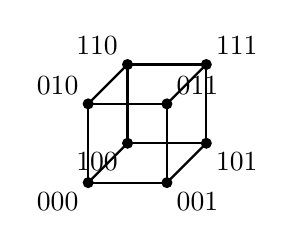
\begin{tikzpicture}[scale=1]
  % Define coordinates for the cube vertices
  \coordinate (A) at (0,0);      % 000
  \coordinate (B) at (1,0);      % 001
  \coordinate (C) at (1,1);      % 011
  \coordinate (D) at (0,1);      % 010
  \coordinate (E) at (0.5,0.5);  % 100
  \coordinate (F) at (1.5,0.5);  % 101
  \coordinate (G) at (1.5,1.5);  % 111
  \coordinate (H) at (0.5,1.5);  % 110

  % Draw edges of the cube
  \draw [thick] (A) -- (B) -- (C) -- (D) -- cycle;       % front square
  \draw [thick] (E) -- (F) -- (G) -- (H) -- cycle;       % back square
  \draw [thick] (A) -- (E);
  \draw [thick] (B) -- (F);
  \draw [thick] (C) -- (G);
  \draw [thick] (D) -- (H);

  % Draw vertices as filled circles
  \fill (A) circle(2pt);
  \fill (B) circle(2pt);
  \fill (C) circle(2pt);
  \fill (D) circle(2pt);
  \fill (E) circle(2pt);
  \fill (F) circle(2pt);
  \fill (G) circle(2pt);
  \fill (H) circle(2pt);

  % Label each vertex with its 3-bit coordinate
  \node[below left] at (A) {$000$};
  \node[below right] at (B) {$001$};
  \node[above right] at (C) {$011$};
  \node[above left] at (D) {$010$};
  \node[below left] at (E) {$100$};
  \node[below right] at (F) {$101$};
  \node[above right] at (G) {$111$};
  \node[above left] at (H) {$110$};
\end{tikzpicture}
\caption{Each vertex corresponds to a 3-bit binary vector. Edges connect vertices that differ in one coordinate (Hamming distance $1$). For example, the neighbors of $000$ (connected directly by an edge) are $001$, $010$, and $100$, which illustrates all vectors at Hamming distance $1$ from $000$.}
\end{figure}

In this cube, one can see how clusters of vectors can be grouped around a given vertex. For instance, as noted, the set $\{000,001,010,100\}$ are all within distance $1$ of $000$ (a Hamming ball of radius $1$ around $000$). If we take a simple code such as $C=\{000,111\}$ (which is the $((3,1))$ repetition code in binary with $n=3$, $k=1$), those codewords correspond to the vertices $000$ and $111$, which are opposite corners of the cube. The minimum distance of this code is $d_C = d_H(000,111) = 3$. The balls of radius $1$ around $000$ and around $111$ (the sets of neighbors each has) do not overlap; in fact, they are separated by at least one bit flip difference. Thus, if at most 1 error occurs during transmission, the received word will remain in the unique “sphere” of radius $1$ around whichever codeword was sent, and decoding can correctly deduce the original codeword. If 2 errors occur, the received word will be distance 2 from the original codeword --- in this case (for $C=\{000,111\}$) a double error could yield a vector like $110$, which is not a codeword but is now only distance 1 away from the \emph{other} codeword $111$. The decoder might misidentify it if it only considers radius $1$ spheres, but it will at least notice an error occurred since $110$ is not itself a codeword. These ideas will be formalized next.



\end{document}
